% Provenance (never printed): see sources/outline_sources.md (Year 1: litho-, bio- and
% chronostratigraphy; boundary stratotypes; mass extinctions as global markers; the
% international chart). Exercise and problem values in the Book 3 scratch calculator
% calc/ch24.py; the chart from figdata/bachelor-1/ics_chart.py (shared ics rows).
% The principles of relative dating, eras and periods are Book 1's (g7 geological-time) and
% are re-founded here. Mass extinctions belong to the biology series (recalled in prose);
% their Earth causes are the Year 2 volume's (phanerozoic-earth). Correlation of logs and
% unconformities are ch. 5's; facies ch. 21's; compaction ch. 23's. Radiometric dating is
% ch. 25's. Sequence stratigraphy, facies models and Walther's law are the Year 3 volume's;
% magnetostratigraphy too: prose pointers only. "Transgression" is explained in prose.
\chapter{A escala estratigráfica}\label{ch:b1:stratigraphic-scale}

Na praia de Itzurun, em Zumaia, na costa basca, as falésias são feitas de camadas finas de
calcário e margas, inclinadas e repetidas por centenas de metros. Em um contato, onde uma
camada pálida de calcário termina e margas vermelhas começam, um disco de bronze gravado com
quatro letras está embutido na rocha (figura abaixo). É um golden spike. Ele fixa, para o
planeta inteiro, o instante em que começa uma divisão do tempo geológico --- o \omterm{def:b1:stratigraphic-scale:chronostratigraphy}{Andar}
Selandiano. Uma rocha na Patagônia ou na Sibéria é selandiana se foi depositada depois do
instante registrado nesse contato e antes do registrado no próximo prego acima na escala.
Este capítulo explica como os geólogos chegaram a precisar de tal marcador: três maneiras
diferentes de dividir uma pilha de rochas, os princípios que as ordenam, as linhas que unem
seções distantes, e a escala internacional que reúne o resultado.

\begin{omfigure}
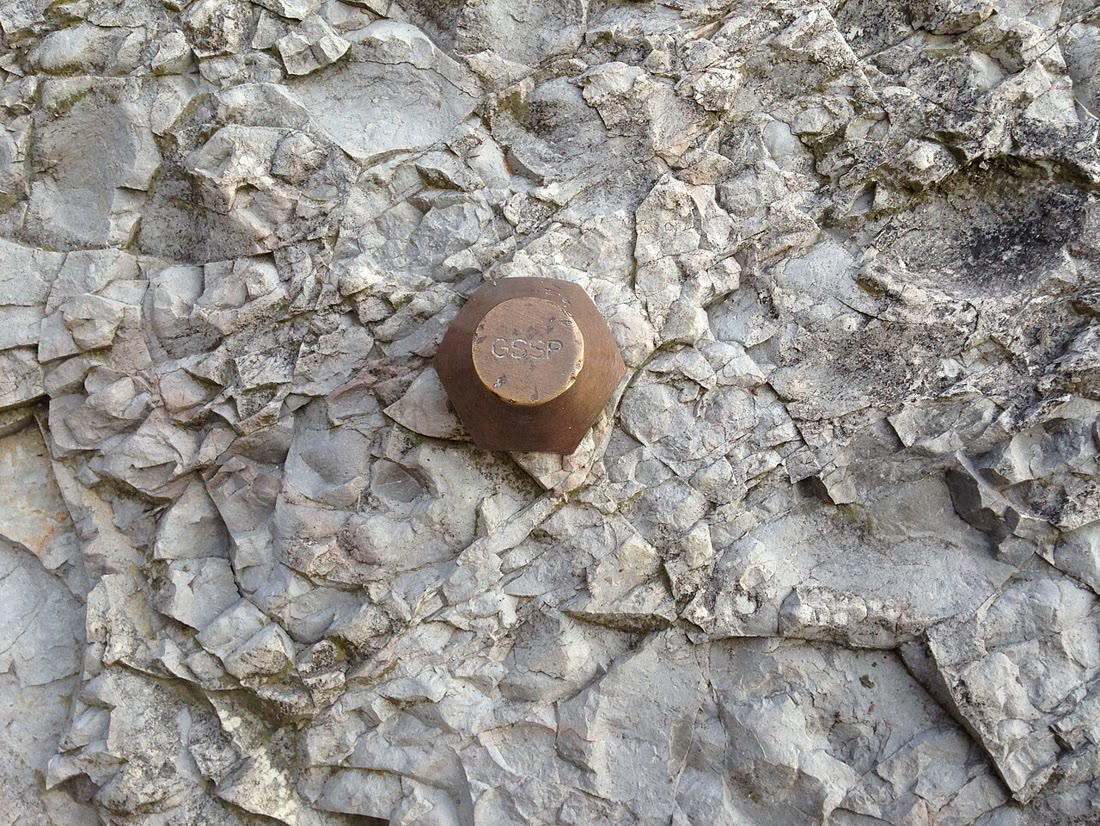
\includegraphics[width=0.62\linewidth]{images/book3/b1-golden-spike-zumaia.jpg}

{\small O golden spike do \omterm{def:b1:stratigraphic-scale:chronostratigraphy}{Andar} Selandiano na seção de Zumaia: um marcador de bronze gravado
GSSP, colocado no topo da camada de calcário mais alta de uma \omterm{def:b1:stratigraphic-scale:lithostratigraphy}{formação}, na base das margas
vermelhas da seguinte. (Josugoni, CC~BY-SA~4.0, via Wikimedia Commons.)}
\label{fig:b1:stratigraphic-scale:zumaia}
\end{omfigure}
% ledger: commons:zumaia-gssp, gssp:selandian

\begin{recall}
Em uma pilha de camadas que não foi virada, cada camada é mais jovem que a de baixo; uma
estrutura que corta rochas é mais jovem que elas; os fósseis mudam das camadas mais antigas
para as mais jovens na mesma ordem em toda parte; a história da Terra é dividida em eras e
períodos geológicos, cada um com uma idade em anos para seu início, reunidos em uma escala
internacional (Livro~1, 7º ano). Um \omterm{def:b1:cross-sections:log}{perfil de sondagem} registra as unidades encontradas em
função da profundidade, e a \omterm{def:b1:cross-sections:log}{correlação} associa as mesmas unidades de perfil a perfil
(\cref{def:b1:cross-sections:log}); uma \omterm{def:b1:cross-sections:unconformity}{discordância} é uma superfície de erosão ou de não
deposição (\cref{def:b1:cross-sections:unconformity}). Uma \omterm{def:b1:clastic-sediments:facies}{fácies sedimentar} é um corpo de
rocha cujos caracteres registram seu ambiente de deposição
(\cref{def:b1:clastic-sediments:facies}). Os livros de biologia descrevem como as espécies
surgem e se extinguem, e as poucas extinções em massa nas quais uma grande parcela de todas
as espécies desapareceu em um curto intervalo de tempo.
\end{recall}

\section{Três maneiras de dividir as rochas}\label{sec:b1:stratigraphic-scale:three}

Um geólogo que descreve uma falésia pode dividir a mesma pilha de camadas de três maneiras:
pelo que as rochas são feitas, pelos fósseis que contêm e pelo tempo durante o qual foram
depositadas. As três divisões respondem a perguntas diferentes, e seus limites não precisam
coincidir. As regras para nomear e definir cada tipo de unidade são fixadas por acordo
internacional.
% ledger: isg:lithostratigraphy

\begin{definition}[Formação, membro, grupo]\label{def:b1:stratigraphic-scale:lithostratigraphy}
Uma \emph{unidade litoestratigráfica}\index{unidade litoestratigráfica} é um corpo de rocha
definido e reconhecido por sua litologia e por sua posição entre outros corpos, qualquer que
seja sua idade. A unidade primária é a \emph{formação}\index{formação (litoestratigráfica)}:
um corpo de rocha suficientemente distinto de seus vizinhos para ser mapeado na escala da
região, em que toda a coluna deve ser dividida. Um \emph{membro}\index{membro (litoestratigráfico)} é uma subdivisão nomeada de uma formação, distinguida por sua litologia;
um \emph{grupo}\index{grupo (litoestratigráfico)} é uma sucessão de duas ou mais formações
com caracteres litológicos significativos em comum. Um nome formal junta um nome geográfico
local ao posto ou à rocha dominante: o Arenito Kell, a Formação Folhelho Mardon.
\end{definition}
% ledger: isg:lithostratigraphy

Uma \omterm{def:b1:stratigraphic-scale:lithostratigraphy}{formação} pode ter menos de um metro de espessura ou vários milhares de metros. Ela se
estende para longe de sua seção-tipo apenas até onde sua litologia pode ser reconhecida, de
modo que seus limites seguem a rocha, não o tempo.
% ledger: isg:lithostratigraphy

\begin{definition}[Biozona, fóssil-índice, datum de primeira aparição]\label{def:b1:stratigraphic-scale:biozone}
Uma \emph{biozona}\index{biozona} é um corpo de estratos definido ou caracterizado pelos
fósseis que contém. Uma \emph{zona de distribuição}\index{zona de distribuição} reúne as
ocorrências conhecidas de um táxon; uma \emph{zona de intervalo}\index{zona de intervalo} é o
corpo de estratos entre dois horizontes fósseis especificados, por exemplo as ocorrências mais
baixas de dois táxons. O \emph{datum de primeira aparição}\index{datum de primeira aparição}
(FAD) de um táxon é o horizonte de sua ocorrência mais baixa, o \emph{datum de última
aparição}\index{datum de última aparição} o de sua mais alta. Um \emph{fóssil-índice}\index{fóssil-índice}
é um táxon usado para reconhecer uma biozona: os melhores são amplamente distribuídos,
abundantes, fáceis de identificar e de vida curta.
\end{definition}
% ledger: isg:biostratigraphy, og:stratigraphy-principles

Um horizonte fóssil não tem espessura; uma \omterm{def:b1:stratigraphic-scale:biozone}{biozona} pode ter alguns metros ou algumas centenas
de metros de espessura, conforme a rapidez com que o sedimento se acumulou enquanto os táxons
viviam. Como as espécies evoluem e nunca reaparecem depois de extintas, a associação de
qualquer idade é única. Alguns dos melhores fósseis-índice são microfósseis, como
foraminíferos e conodontes: amplamente distribuídos, abundantes e pequenos o bastante para
serem recuperados dos cascalhos de perfuração de um poço.
% ledger: isg:biostratigraphy, og:stratigraphy-principles

\begin{definition}[Unidades cronoestratigráficas e geocronológicas]\label{def:b1:stratigraphic-scale:chronostratigraphy}
Uma \emph{unidade cronoestratigráfica}\index{unidade cronoestratigráfica} é o corpo de todas as
rochas formadas durante um dado intervalo de tempo geológico, e apenas durante ele; seus
limites são superfícies de igual idade. O próprio intervalo de tempo é uma \emph{unidade
geocronológica}\index{unidade geocronológica}. As categorias, da menor, são o
\emph{andar}\index{andar (cronoestratigráfico)} (seu tempo: uma idade), a
\emph{série}\index{série (cronoestratigráfica)} (uma época), o \emph{sistema}\index{sistema (cronoestratigráfico)} (um período), o eratema (uma era) e o eonotema (um éon); cada unidade é
formada por várias unidades consecutivas da categoria abaixo.
\end{definition}
% ledger: isg:chronostratigraphy

As duas palavras descrevem a mesma divisão vista como rocha ou como tempo
(\cref{tab:b1:stratigraphic-scale:ranks}): rochas do \omterm{def:b1:stratigraphic-scale:chronostratigraphy}{Sistema} Jurássico foram depositadas
durante o Período Jurássico, e a \omterm{def:b1:stratigraphic-scale:chronostratigraphy}{Série} Jurássica Inferior, durante a Época Jurássica Inferior.
O \omterm{def:b1:stratigraphic-scale:chronostratigraphy}{andar} é a menor unidade reconhecida em todo o mundo.
% ledger: isg:chronostratigraphy, chart:danian

\begin{table}[htbp]
\centering
\begin{tabular}{lll}
\hline
\omterm{def:b1:stratigraphic-scale:chronostratigraphy}{unidade cronoestratigráfica} & \omterm{def:b1:stratigraphic-scale:chronostratigraphy}{unidade geocronológica} & exemplo \\
\hline
eonotema & éon    & Fanerozoico \\
eratema  & era    & Cenozoico \\
\omterm{def:b1:stratigraphic-scale:chronostratigraphy}{sistema}  & período & Paleógeno \\
\omterm{def:b1:stratigraphic-scale:chronostratigraphy}{série}    & época  & Paleoceno \\
\omterm{def:b1:stratigraphic-scale:chronostratigraphy}{andar}    & idade  & Daniano (\qtyrange{66.00}{61.66}{\Ma}) \\
\hline
\end{tabular}
\caption{As categorias das \omterm{def:b1:stratigraphic-scale:chronostratigraphy}{unidades cronoestratigráficas} e geocronológicas, com as unidades
que contêm o Daniano, o primeiro \omterm{def:b1:stratigraphic-scale:chronostratigraphy}{andar} do Cenozoico.}
\label{tab:b1:stratigraphic-scale:ranks}
\end{table}
% ledger: isg:chronostratigraphy, chart:danian

\section{Os princípios e a correlação}\label{sec:b1:stratigraphic-scale:principles}

Antes que qualquer rocha pudesse ser datada em anos, a ordem dos eventos foi lida nas próprias
rochas. Os princípios básicos da estratigrafia foram expostos em 1669 por Nicolau Steno; entre
1785 e 1800, Hutton e William Smith acrescentaram o uso das camadas como intervalos de tempo e
de seus fósseis para reconhecê-las.
% ledger: og:stratigraphy-principles, usgs:hutton-smith

\begin{definition}[Princípios da estratigrafia]\label{def:b1:stratigraphic-scale:principles}
\begin{enumerate}
  \item O \emph{princípio da superposição}\index{superposição, princípio da}: em uma sequência
        de camadas sedimentares que não foi invertida, cada camada é mais jovem que aquela
        sobre a qual repousa.
  \item O \emph{princípio da horizontalidade original}\index{horizontalidade original, princípio         da}: sedimentos e derrames de lava são depositados horizontalmente, ou quase ---
        levemente inclinados nas bordas de uma bacia.
  \item O \emph{princípio da continuidade lateral}\index{continuidade lateral, princípio da}:
        dentro de uma bacia, uma camada se estende continuamente em todas as direções até
        afinar na borda da bacia ou contra um obstáculo; uma camada cortada por um vale
        continua do outro lado.
  \item O \emph{princípio das relações de corte}\index{relações de corte, princípio das}: um
        corpo ou uma estrutura que corta rochas --- um dique, uma falha, uma superfície de
        erosão --- é mais jovem que as rochas que corta.
  \item O \emph{princípio da sucessão faunística}\index{sucessão faunística, princípio da}:
        táxons fósseis se sucedem na mesma ordem em toda região, de modo que rochas com a
        mesma associação são da mesma idade.
\end{enumerate}
\end{definition}
% ledger: og:stratigraphy-principles, eli:relative-dating, usgs:fossil-succession, isg:chronostratigraphy

Os princípios não são igualmente fortes. A superposição dá uma ordem que todos os outros
métodos devem respeitar. A horizontalidade original é o que faz de uma camada inclinada um
registro de deformação posterior. A continuidade lateral é o que permite a um geólogo
desenhar a mesma camada dos dois lados de um vale e, dentro de uma distância limitada, um
plano de acamamento traçado no terreno é a melhor linha de igual idade que existe. A sucessão
faunística é a que atravessa os oceanos; é o tema dos próximos parágrafos.
% ledger: isg:chronostratigraphy, og:stratigraphy-principles

\subsection*{Correlação por biozonas}

A \omterm{def:b1:cross-sections:log}{correlação} por fósseis compara a ordem das primeiras e últimas aparições em duas seções
(figura abaixo). As duas não são igualmente confiáveis. O fóssil mais alto de um táxon
encontrado em uma seção depende de quantos foram preservados: onde são raros, o último
encontrado pode estar bem abaixo do nível em que o táxon realmente desapareceu, e um fóssil
erodido e redepositado pode aparecer acima dele. Uma primeira aparição também pode ser
deslocada, mas um táxon amplamente distribuído que se espalhou depressa é atingido quase no
mesmo nível em toda uma bacia.
% ledger: isg:biostratigraphy

\begin{omfigure}
\begin{tikzpicture}[font=\footnotesize, y=0.13cm]
  % section 1: 40 m, sandstone 0-14, shale 14-40
  \fill[lith sandstone] (0,0) rectangle (0.8,14);
  \fill[lith shale] (0,14) rectangle (0.8,40);
  \draw[black!70] (0,0) rectangle (0.8,40);
  \node[anchor=south, font=\small] at (1.4,41.5) {seção 1};
  \foreach \x/\a/\b/\t in {1.1/0/27/a, 1.4/10/34/b, 1.7/20/40/c, 2.0/30/40/d} {
    \draw[line width=2.2pt, omThm] (\x,\a) -- (\x,\b);
    \node[anchor=base, font=\scriptsize] at (\x,-4.5) {\t};
  }
  \foreach \y/\z in {5/a, 15/b, 25/c, 35/d}
    \node[anchor=east, font=\scriptsize] at (-0.1,\y) {zona \z};
  \foreach \y in {10,20,30} \draw[black!50] (-1.3,\y) -- (0,\y);
  % scale bar
  \draw[thick] (-1.5,0) -- (-1.5,10) node[midway, anchor=east, font=\scriptsize] {\qty{10}{m}};
  % section 2: 24 m, sandstone 0-3, shale 3-24
  \begin{scope}[xshift=7cm]
    \fill[lith sandstone] (0,0) rectangle (0.8,3);
    \fill[lith shale] (0,3) rectangle (0.8,24);
    \draw[black!70] (0,0) rectangle (0.8,24);
    \node[anchor=south, font=\small] at (1.4,25.5) {seção 2};
    \foreach \x/\a/\b/\t in {1.1/0/13/a, 1.4/6/20/b, 1.7/12/24/c, 2.0/18/24/d} {
      \draw[line width=2.2pt, omThm] (\x,\a) -- (\x,\b);
      \node[anchor=base, font=\scriptsize] at (\x,-4.5) {\t};
    }
    \foreach \y/\z in {3/a, 9/b, 15/c, 21/d}
      \node[anchor=west, font=\scriptsize] at (2.3,\y) {zona \z};
    \foreach \y in {6,12,18} \draw[black!50] (0.8,\y) -- (2.3,\y);
  \end{scope}
  % correlation of the first appearances
  \foreach \u/\v/\t in {10/6/b, 20/12/c, 30/18/d}
    \draw[densely dashed, omThm!70!black] (2.15,\u) -- (6.85,\v)
      node[pos=0.5, fill=white, inner sep=1pt, font=\scriptsize] {FAD \t};
\end{tikzpicture}

{\small Um gráfico de distribuição e uma \omterm{def:b1:cross-sections:log}{correlação} por \omterm{def:b1:stratigraphic-scale:biozone}{biozonas} (táxons inventados \emph{a} a
\emph{d}). As barras grossas são as distribuições dos táxons em cada seção. Três \omterm{def:b1:stratigraphic-scale:biozone}{zonas de
intervalo} são delimitadas pelas primeiras aparições de \emph{b}, \emph{c} e \emph{d}, que são
unidas de seção a seção (tracejado). A última aparição de \emph{a} cai na parte superior da
zona~\emph{c} na seção~1 e perto de sua base na seção~2: é um guia pior. As zonas são mais
finas na seção~2, onde o sedimento se acumulou mais lentamente.}
\label{fig:b1:stratigraphic-scale:range-chart}
\end{omfigure}

\begin{method}[Correlação de seções por biozonas]\label{met:b1:stratigraphic-scale:biozones}
\begin{enumerate}
  \item Plote, para cada seção, a distribuição de cada táxon em função da altura: da sua
        ocorrência mais baixa até a mais alta.
  \item Escolha os horizontes fósseis que definem as zonas --- de preferência primeiras
        aparições de táxons amplamente distribuídos e independentes da fácies.
  \item Desenhe os limites das zonas em cada seção nesses horizontes.
  \item Una os mesmos horizontes de seção a seção; verifique que as linhas não se cruzam,
        como exige a superposição.
  \item Leia, entre duas linhas, a espessura de cada zona em cada seção; onde uma zona
        estiver ausente, procure uma \omterm{def:b1:cross-sections:unconformity}{discordância} ou uma mudança de fácies antes de concluir
        que o táxon não existe.
\end{enumerate}
\end{method}

Uma \omterm{def:b1:stratigraphic-scale:biozone}{biozona} só é tão boa quanto a independência de seus fósseis em relação ao ambiente. Um
bivalve que viveu apenas em praias arenosas só é encontrado em arenitos; segui-lo de seção a
seção é seguir o arenito, não o tempo. A \omterm{def:b1:cross-sections:log}{correlação} bioestratigráfica não é, portanto,
necessariamente uma \omterm{def:b1:cross-sections:log}{correlação} de tempo: ela pode seguir uma fácies cuja idade muda de lugar
para lugar.
% ledger: isg:biostratigraphy

\subsection*{Limites que atravessam o tempo}

Sedimentos diferentes são depositados ao mesmo tempo em lugares diferentes: areia na praia,
lama no mar aberto, calcário mais adiante em uma plataforma sem areia. Uma linha de igual
idade passa, portanto, de uma litologia para outra. Inversamente, um limite litológico traçado
através de uma bacia não precisa ser de forma alguma uma linha de igual idade.
% ledger: og:stratigraphy-principles, isg:chronostratigraphy

\begin{definition}[Limite diácrono]\label{def:b1:stratigraphic-scale:diachronous}
Um limite é \emph{diácrono}\index{limite diácrono} quando sua idade muda de lugar para lugar
ao longo dele. Os limites de formações e de fácies são em geral diácronos; os limites das
\omterm{def:b1:stratigraphic-scale:chronostratigraphy}{unidades cronoestratigráficas} não são, por definição.
\end{definition}
% ledger: isg:lithostratigraphy, isg:chronostratigraphy, isg:biostratigraphy

O caso clássico é uma transgressão: o \omterm{def:b1:diagenesis-basins:eustasy}{nível relativo do mar} sobe mais depressa que o sedimento
consegue preencher o espaço criado, e a linha de costa avança para o interior. A areia da praia
é depositada na linha de costa a cada instante, de modo que um lençol de arenito se espalha
para o interior com ela; a lama de mar aberto se sobrepõe. O topo do arenito é então o rastro
da linha de costa em movimento: jovem para o interior, velho em direção ao mar (figura
abaixo). A ordem das fácies vista em uma seção vertical --- arenito sob folhelho sob calcário
--- repete sua ordem através da plataforma em um instante; o Livro~5 faz disso a base de
seus modelos de fácies.
% ledger: og:stratigraphy-principles, isg:lithostratigraphy

\begin{omfigure}
\begin{tikzpicture}[font=\footnotesize, x=1cm, y=1cm]
  % basement surface B(x) = 1.6 (1 - x/14), rising towards the land on the left
  \fill[lith granite] (0,-0.5) -- (0,1.6) -- (14,0) -- (14,-0.5) -- cycle;
  \fill[lith sandstone] (0,1.6) -- (14,0) -- (14,0.5) -- (0,2.1) -- cycle;
  \fill[lith shale] (0,2.1) -- (14,0.5) -- (14,1.5) -- (0,3.1) -- cycle;
  \fill[lith limestone] (0,3.1) -- (14,1.5) -- (14,3.6) -- (0,3.6) -- cycle;
  \draw[unconformity] (0,1.6) -- (14,0);
  \draw[black!70] (0,2.1) -- (14,0.5) (0,3.1) -- (14,1.5);
  \draw[black!70] (0,-0.5) rectangle (14,3.6);
  % time lines: horizontal, from the basement (or the left edge) to the right edge
  \foreach \y/\t in {0.6/1, 1.1/2, 1.6/3, 2.1/4, 2.6/5, 3.1/6} {
    \pgfmathsetmacro{\xs}{max(0, 14*(1-\y/1.6))}
    \draw[omThm, thick, densely dashed] (\xs,\y) -- (14,\y) node[anchor=west, text=black] {$t_\t$};
  }
  % two sections
  \foreach \x/\n in {3/1, 11/2} {
    \draw[very thick, black] (\x,-0.5) -- (\x,3.6);
    \node[anchor=south, font=\small] at (\x,3.65) {seção \n};
  }
  \node[fill=white, inner sep=1pt, font=\scriptsize] at (5.6,1.21) {arenito};
  \node[fill=white, inner sep=1pt] at (12.6,1.2) {folhelho};
  \node[fill=white, inner sep=1pt] at (7.0,3.25) {calcário};
  \node[fill=white, inner sep=1pt] at (12.0,-0.25) {embasamento};
  \draw[-{Stealth}, thick] (5.6,4.35) -- (3.6,4.35) node[anchor=east] {terra};
  \draw[-{Stealth}, thick] (8.4,4.35) -- (10.4,4.35) node[anchor=west] {mar};
\end{tikzpicture}

{\small Um lençol de arenito depositado durante uma transgressão (esquemático, escala vertical
exagerada). As linhas tracejadas $t_1$ a $t_6$ unem pontos de igual idade, $t_1$ a mais
antiga. Onde uma encontra o embasamento, ela começa na linha de costa de seu tempo; em direção
ao mar passa de areia a lama e, nas mais jovens, a calcário. O topo do arenito fica entre
$t_1$ e $t_2$ na seção~2, mas entre $t_3$ e $t_4$ na seção~1: o limite de \omterm{def:b1:stratigraphic-scale:lithostratigraphy}{formação} é
\omterm{def:b1:stratigraphic-scale:diachronous}{diácrono}, mais jovem em direção à terra.}
\label{fig:b1:stratigraphic-scale:diachronous}
\end{omfigure}

Com que rapidez a idade do limite muda ao longo dele? Em uma planície costeira que sobe
suavemente para o interior, a resposta é uma questão de geometria.

\begin{proposition}[Velocidade de uma transgressão]\label{prop:b1:stratigraphic-scale:transgression}
Uma planície costeira sobe para o interior com a inclinação uniforme $s$, e o \omterm{def:b1:diagenesis-basins:eustasy}{nível relativo
do mar} sobe à taxa constante $R$, sem sedimento acrescentado na costa. A linha de costa então
se move para o interior à velocidade
\[
  u = \frac{R}{s},
\]
e um limite que segue a linha de costa é mais jovem, em um ponto a uma distância $d$ mais para
o interior, por $\Delta t = d/u = d\,s/R$.
\end{proposition}

\begin{proof}
Tome $x$ como a distância para o interior a partir de um ponto fixo e $z$ como a altura; a
planície é a reta $z = s x$, e a superfície do mar no tempo $t$ é
$z = z_0 + R t$. A linha de costa está onde eles se encontram: $s\,x(t) = z_0 + R t$, logo
$x(t) = (z_0 + R t)/s$ e $\mathrm dx/\mathrm dt = R/s$. A linha de costa alcança um ponto a
uma distância $d$ mais para o interior após o tempo $d/u = d\,s/R$.
\end{proof}

A razão é grande porque as planícies costeiras são quase planas. Uma elevação de \qty{10}{m}
por milhão de anos sobre uma planície com inclinação de $1$ em $2000$ desloca a costa
\qty{20}{km} para o interior por milhão de anos; um topo de arenito que parece uma só
superfície em uma falésia é então um milhão de anos mais jovem a \qty{20}{km} para o
interior. Sedimento trazido à costa retarda a transgressão ou a reverte.

\subsection*{Linhas de igual idade}

O que correlaciona o tempo, então, se a litologia não o faz e os fósseis só aproximadamente?
As melhores linhas são feitas por eventos que deixam um rastro em toda parte ao mesmo tempo.
Uma cinza vulcânica cai sobre uma grande área em um instante, do ponto de vista geológico, e
assenta-se sobre areia, lama e calcário igualmente: uma camada de cinza é uma linha de igual
idade que atravessa limites de fácies, e muitas vezes pode ser datada em anos pelos métodos de
\cref{ch:b1:radiometric-methods}. As inversões do campo magnético da Terra, tratadas no
Livro~5, são registradas em rochas de muitos tipos e podem ser reconhecidas em todo o mundo
uma vez conhecida sua ordem; o mesmo ocorre com as mudanças bruscas nos isótopos do carbono,
como a que marca a base do Ipresiano (\cref{tab:b1:stratigraphic-scale:gssps}). Entre dois
níveis datados, a idade de qualquer camada é estimada supondo que o sedimento se acumulou a
uma taxa constante.
% ledger: isg:chronostratigraphy

\begin{proposition}[Idade entre dois níveis datados]\label{prop:b1:stratigraphic-scale:interpolation}
Duas camadas nas alturas $z_1 < z_2$ de uma seção contínua têm as idades $t_1 > t_2$. Se o
sedimento se acumulou a uma taxa constante entre elas, um nível na altura $z$ entre elas tem a
idade
\[
  t = t_1 - f\,(t_1 - t_2), \qquad f = \frac{z - z_1}{z_2 - z_1},
\]
e a taxa de acumulação é $r = (z_2 - z_1)/(t_1 - t_2)$. Se as duas idades carregam as
incertezas padrão independentes $\sigma_1$ e $\sigma_2$, a idade interpolada carrega a incerteza
\[
  \sigma_t = \sqrt{(1 - f)^2 \sigma_1^2 + f^2 \sigma_2^2}.
\]
\end{proposition}

\begin{proof}
À taxa constante $r$, a altura cresce linearmente com o tempo: $z - z_1 = r\,(t_1
- t)$, já que as idades diminuem para cima. Em $z_2$, $z_2 - z_1 = r\,(t_1 - t_2)$, o que
dá $r$; dividindo as duas relações obtém-se $t_1 - t = f\,(t_1 - t_2)$. A idade é a
combinação linear $t = (1 - f)\,t_1 + f\,t_2$ de duas quantidades independentes; a variância
de $a X + b Y$ para $X$ e $Y$ independentes é $a^2
\operatorname{Var} X + b^2 \operatorname{Var} Y$, o que dá $\sigma_t$.
\end{proof}

A incerteza é menor entre as duas camadas datadas, e ali nunca é maior que a maior entre
$\sigma_1$ e $\sigma_2$. O limite real é a suposição: o sedimento se acumula em pulsos, pode
parar em quebras escondidas, e se compacta de modo diferente na areia e na lama
(\cref{prop:b1:diagenesis-basins:solid}), de modo que a idade interpolada não é melhor que a
regularidade da seção.

\section{Estratótipos de limite}\label{sec:b1:stratigraphic-scale:gssp}

Uma \omterm{def:b1:stratigraphic-scale:chronostratigraphy}{unidade cronoestratigráfica} é definida na rocha antes de ser datada. A prática antiga
descrevia cada \omterm{def:b1:stratigraphic-scale:chronostratigraphy}{andar} por uma seção-tipo de toda a unidade; mas o topo de uma seção-tipo e a
base da seguinte, escolhidas em lugares diferentes, podiam deixar entre elas uma lacuna de
tempo não atribuído ou se sobrepor. A prática moderna define apenas o limite inferior de cada
unidade em um ponto de uma seção; o limite superior é o limite inferior da unidade seguinte.
Nenhum intervalo de tempo pode então cair entre duas unidades ou pertencer a ambas.
% ledger: isg:stratotype, isg:chronostratigraphy

\begin{definition}[Estratótipo de limite, estratótipo de unidade, GSSP]\label{def:b1:stratigraphic-scale:gssp}
Um \emph{estratótipo}\index{estratótipo} é a seção de rocha designada que serve de padrão de
referência para uma unidade ou um limite. Um \emph{estratótipo de unidade}\index{estratótipo de unidade} é a seção-tipo de uma unidade inteira; um \emph{estratótipo de limite}\index{estratótipo de limite} é a seção que contém o ponto específico que define um limite entre duas unidades. Uma
\emph{seção e ponto estratotípico global de limite}\index{seção e ponto estratotípico global de limite (GSSP)} (GSSP) é o estratótipo de limite de uma unidade da escala cronoestratigráfica
internacional: um único ponto em uma única seção, escolhido por acordo internacional, que define
a base de um \omterm{def:b1:stratigraphic-scale:chronostratigraphy}{andar} e de toda unidade maior que começa com ele.
\end{definition}
% ledger: isg:stratotype, isg:chronostratigraphy, gssp:protocol

O GSSP é um ponto na rocha, não uma idade. Sua idade em anos é a que a melhor datação desse
ponto der, e pode ser refinada sem que o ponto se mova. A seção é escolhida para tornar o ponto
encontrável em outros lugares: deposição contínua através do limite (nunca em uma \omterm{def:b1:cross-sections:unconformity}{discordância},
onde o tempo faltante tornaria o limite ambíguo), de preferência marinha, rica em fósseis bem
preservados de táxons amplamente distribuídos, sem mudança de fácies no nível, pouco deformada
ou alterada, acessível e protegida. Acima de tudo, o ponto é colocado em um nível que coincide
com um sinal escolhido --- em geral a primeira aparição de um táxon --- dentro de um intervalo
rico em outros sinais (camadas de cinza, inversões magnéticas, mudanças isotópicas) pelos quais
o nível pode ser reconhecido à distância. Um marcador permanente, o golden spike, é colocado
no ponto.
% ledger: isg:chronostratigraphy, isg:stratotype, gssp:protocol

\begin{inthefield}[Como um limite é escolhido]
Um limite é estudado por um grupo de trabalho da subcomissão encarregada do \omterm{def:b1:stratigraphic-scale:chronostratigraphy}{sistema}, que
compara seções candidatas, descreve-as camada por camada, amostra seus fósseis, camadas de cinza
e isótopos, e escreve uma proposta. Uma proposta precisa de uma supermaioria --- mais de
\qty{60}{\%} --- dos membros votantes da subcomissão, cerca de vinte especialistas; ela passa
então aos membros votantes da Comissão Internacional de Estratigrafia, aos dirigentes e aos
presidentes de suas dezessete subcomissões, e por fim ao comitê executivo da União Internacional
de Ciências Geológicas, cuja aprovação a ratifica. Os resultados são publicados, o marcador é
colocado na rocha, e nenhuma mudança em um limite recém-estabelecido pode ser proposta por dez anos.
\end{inthefield}
% ledger: gssp:protocol

\begin{table}[htbp]
\centering
\small
\begin{tabular}{>{\raggedright\arraybackslash}p{2.4cm}>{\raggedright\arraybackslash}p{1.2cm}>{\raggedright\arraybackslash}p{3.7cm}>{\raggedright\arraybackslash}p{5.6cm}c}
\hline
base de & idade (\unit{\Ma}) & seção & marcador do ponto & ratificado \\
\hline
Fortuniano (Cambriano) & 538.8 & Fortune Head, Terra Nova, Canadá & primeira aparição do icnofóssil \emph{Trichophycus pedum} & 1992 \\
Lochkoviano (Devoniano) & 419.62 & Klonk, perto de Praga, República Tcheca & primeira aparição do graptólito \emph{Monograptus uniformis} & 1972 \\
Induano (Triássico) & 251.902 & Meishan, Zhejiang, China & primeira aparição do conodonte \emph{Hindeodus parvus}, base da camada~27c & 2001 \\
Daniano (Paleógeno) & 66.00 & Oued Djerfane, El Kef, Tunísia & base de uma argila escura de fronteira de \qty{50}{cm}; anomalia de irídio & 1991 \\
Selandiano & 61.66 & Zumaia, Espanha & base das margas vermelhas; segunda radiação de um grupo de nanofósseis & 2008 \\
Ipresiano (Eoceno) & 56.00 & Dababiya, perto de Luxor, Egito & base de uma excursão de isótopos de carbono & 2003 \\
Chibaniano & 0.774 & Chiba, Japão & base de uma tefra, logo abaixo de uma inversão magnética & 2020 \\
Meghalayano & 0.0042 & Caverna Mawmluh, Meghalaya, Índia & um nível a \qty{7.45}{mm} de profundidade em um espeleotema & 2018 \\
\hline
\end{tabular}
\caption{Oito GSSPs. Os marcadores são primeiras aparições de táxons, uma anomalia geoquímica,
uma excursão isotópica, uma inversão magnética e um evento climático registrado em um depósito
de caverna.}
\label{tab:b1:stratigraphic-scale:gssps}
\end{table}
% ledger: gssp:fortunian, gssp:lochkovian, gssp:induan, gssp:danian, gssp:selandian, gssp:ypresian, gssp:chibanian, gssp:meghalayan

\Cref{tab:b1:stratigraphic-scale:gssps} mostra quão variados são os sinais escolhidos. As
fronteiras paleozoicas e mesozoicas da tabela apoiam-se em primeiras aparições de fósseis, um
graptólito e um conodonte; na base do Cambriano o fóssil é um icnofóssil, a marca deixada no
sedimento pela atividade de um animal, e não o animal em si. Nos exemplos cenozoicos os sinais
são químicos e físicos: o irídio do Daniano, a excursão de isótopos de carbono do Ipresiano, a
inversão magnética que fica \qty{1.1}{m} acima do ponto do Chibaniano. O limite mais jovem da
tabela não está em rocha marinha de forma alguma: a base do Meghalayano é um nível dentro de um
espeleotema, um depósito crescido em uma caverna, registrando um evento climático de 4200 anos
atrás.
% ledger: gssp:fortunian, gssp:danian, gssp:ypresian, gssp:chibanian, gssp:meghalayan

\begin{dated}{2026}
% ledger: gssp:count, chart:stage-count
Em outubro de 2026 a tabela da Comissão Internacional de Estratigrafia listava 80 GSSPs
ratificados e outros dois propostos. O primeiro foi ratificado em 1972, em Klonk; o mais
recente, em 2024, quando dois limites do Siluriano, até então definidos no País de Gales, foram
transferidos para novas seções na Espanha e na República Tcheca. Dos 101 \omterm{def:b1:stratigraphic-scale:chronostratigraphy}{andares} do Fanerozoico
na escala, 21 ainda não tinham um GSSP ratificado; suas bases são provisórias.
\end{dated}

Abaixo do Fanerozoico, a escala é em geral dividida de outra maneira. Exceto por seu \omterm{def:b1:stratigraphic-scale:chronostratigraphy}{sistema}
mais jovem, o Ediacarano, o Pré-Cambriano é cortado em idades redondas escolhidas por acordo ---
as divisões são definidas em anos, não por pontos na rocha.
% ledger: isg:chronostratigraphy

\section{Extinções em massa como marcadores}\label{sec:b1:stratigraphic-scale:extinctions}

Os livros de biologia descrevem as extinções em massa como momentos em que uma grande parcela
das espécies desapareceu em um intervalo geologicamente curto. Para a estratigrafia, tal evento
é uma dádiva: um horizonte encontrado em todos os continentes e em todos os oceanos, através do
qual as associações fósseis mudam por completo. Duas delas delimitam as três eras do
Fanerozoico.
% ledger: schulte:kpg, burgess:end-permian

\subsection*{O fim do Cretáceo}

Em 1980, L.~W.~Alvarez, W.~Alvarez, F.~Asaro e H.~V.~Michel mediram o irídio --- um dos metais
do grupo da platina, empobrecido na \omterm{def:b1:layered-earth:layers}{crosta} terrestre em comparação com sua abundância no
cosmos --- em calcários de mar profundo através do limite entre o Cretáceo e o Terciário, hoje
o limite entre o Cretáceo e o Paleógeno, o limite K--Pg. Encontraram-no enriquecido cerca de 30
vezes acima do fundo na Itália, 160 vezes na Dinamarca e 20 vezes na Nova Zelândia, exatamente
no nível das extinções. Propuseram que um \omterm{def:b1:comparative-planetology:small-bodies}{asteroide} de $\qty{10}{km}$ de diâmetro, para mais ou
para menos quatro, havia atingido a Terra e lançado na atmosfera cerca de 60 vezes sua própria
massa de rocha pulverizada; a poeira teria se espalhado pelo mundo e escurecido o céu. A argila
no limite, observaram, difere quimicamente da argila dos calcários acima e abaixo.
% ledger: alvarez:iridium

Trabalhos posteriores ligaram o limite a um só impacto, Chicxulub. A datação argônio--argônio
situa esse impacto e o limite com suas extinções a menos de \num{32000} anos um do outro, e uma
revisão das evidências concluiu que o impacto desencadeou a extinção, que também caiu dentro do
tempo de um grande derrame de basalto na Índia. O GSSP da base do Daniano --- a base do
Paleógeno e de todo o Cenozoico --- é colocado na base da argila escura de fronteira em El Kef,
na Tunísia, na anomalia de irídio. O mesmo limite pode ser visto em terra, no Colorado (figura
abaixo).
% ledger: renne:kpg, schulte:kpg, gssp:danian, commons:kt-tlsp

\begin{omfigure}
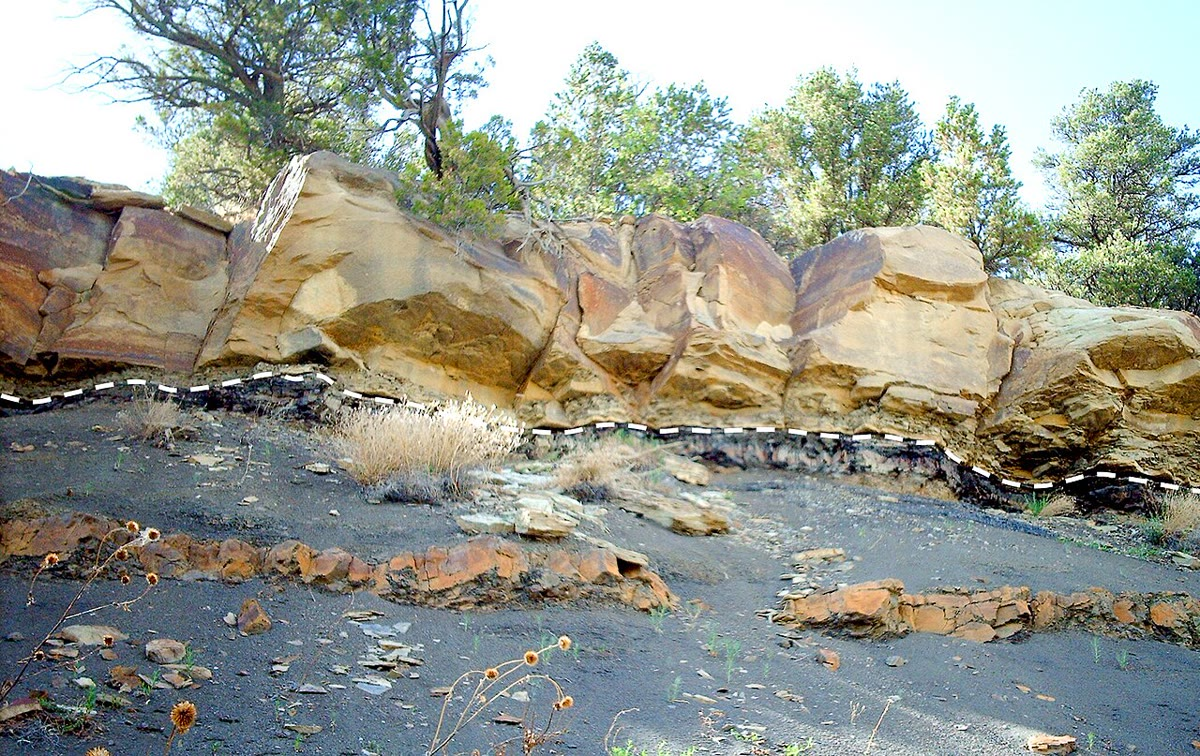
\includegraphics[width=0.78\linewidth]{images/book3/b1-kpg-boundary-trinidad.jpg}

{\small O limite entre o Cretáceo e o Paleógeno, marcado pela linha tracejada, no Parque
Estadual do Lago Trinidad, Colorado: arenito acima, camadas escuras abaixo e ao longo do
limite. (Nationalparks, CC~BY-SA~2.5, via Wikimedia Commons; a linha tracejada está no
original.)}
\label{fig:b1:stratigraphic-scale:kpg}
\end{omfigure}
% ledger: commons:kt-tlsp

\subsection*{O fim do Permiano}

A extinção no fim do Permiano foi a mais severa perda de vida marinha e terrestre dos últimos
meio bilhão de anos. Em Meishan, na China, a seção que contém o GSSP da base do Triássico, cinco
camadas de cinza foram datadas pelo método urânio--chumbo em zircão. Elas situam a extinção
entre \qty[uncertainty-mode=separate]{251.941(37)}{\Ma} e
\qty[uncertainty-mode=separate]{251.880(31)}{\Ma}: um intervalo de
\num[uncertainty-mode=separate]{60 \pm 48} mil anos. Uma queda negativa brusca de
\qty{3}{\permil} nos isótopos de carbono dos carbonatos a precede, e o ciclo do carbono
permaneceu instável por cerca de \num{500} mil anos.
% ledger: burgess:end-permian, gssp:induan

A própria base do Triássico, \qty[uncertainty-mode=separate]{251.902(24)}{\Ma}, não é colocada
na extinção, mas na primeira aparição do conodonte \emph{Hindeodus parvus}, um nível que cai
dentro do intervalo da extinção datado em Meishan. Uma extinção é um conjunto de últimas
aparições, que a preservação embaça; uma primeira aparição de uma espécie bem conhecida faz uma
linha mais nítida. As causas das duas extinções --- um impacto, as grandes províncias de basalto
--- são o assunto do Livro~4.
% ledger: gssp:induan, isg:biostratigraphy, burgess:end-permian

\section{A escala cronoestratigráfica internacional}\label{sec:b1:stratigraphic-scale:chart}

A Carta Cronoestratigráfica Internacional reúne todas as unidades, dos eonotemas aos \omterm{def:b1:stratigraphic-scale:chronostratigraphy}{andares},
em uma só tabela: seus nomes, a base de cada uma em milhões de anos com sua incerteza, uma marca
para cada base definida por um GSSP ratificado, e uma cor padrão para cada unidade, a da
Comissão para a Carta Geológica do Mundo. A parte fanerozoica, reduzida às suas eras e
períodos, é desenhada abaixo com base nos próprios valores da carta.
% ledger: ics:base.Paleozoic, ics:colour.Paleozoic, gssp:count

\begin{omfigure}
\begin{tikzpicture}[font=\footnotesize]
\begin{axis}[y dir=reverse, ymin=0, ymax=538.8, xmin=0, xmax=6.2,
  width=6.6cm, height=11cm, scale only axis, clip=false,
  axis x line=none, axis y line*=left, ytick={0,100,...,500},
  ylabel={idade (\unit{\Ma})}, tick label style={font=\scriptsize}]
  \pgfplotsinvokeforeach{Paleozoic,Mesozoic,Cenozoic,Cambrian,Ordovician,Silurian,Devonian,Carboniferous,Permian,Triassic,Jurassic,Cretaceous,Paleogene,Neogene,Quaternary}{
    \addplot[fill=ics#1, draw=black!70, line width=0.3pt] table[x=x, y=age] {figdata/out/bachelor-1-ics_chart-bar-#1.dat};}
  \node[anchor=center, rotate=90, font=\scriptsize\bfseries] at (axis cs:0.5,395.351) {Paleozoico};
  \node[anchor=center, rotate=90, font=\scriptsize\bfseries] at (axis cs:0.5,158.951) {Mesozoico};
  \node[anchor=center, rotate=90, font=\scriptsize\bfseries] at (axis cs:0.5,33) {Cenozoico};
  \node[anchor=center, font=\scriptsize] at (axis cs:2,512.825) {Cambriano};
  \node[anchor=center, font=\scriptsize] at (axis cs:2,464.975) {Ordoviciano};
  \node[anchor=center, font=\scriptsize] at (axis cs:2,431.36) {Siluriano};
  \node[anchor=center, font=\scriptsize] at (axis cs:2,389.24) {Devoniano};
  \node[anchor=center, font=\scriptsize] at (axis cs:2,328.88) {Carbonífero};
  \node[anchor=center, font=\scriptsize] at (axis cs:2,275.401) {Permiano};
  \node[anchor=center, font=\scriptsize] at (axis cs:2,226.651) {Triássico};
  \node[anchor=center, font=\scriptsize] at (axis cs:2,172.25) {Jurássico};
  \node[anchor=center, font=\scriptsize] at (axis cs:2,104.55) {Cretáceo};
  \node[anchor=center, font=\scriptsize] at (axis cs:2,44.52) {Paleógeno};
  \node[anchor=center, font=\scriptsize] at (axis cs:2,12.81) {Neógeno};
  \addplot[mark=-, mark size=3pt, only marks, nodes near coords, point meta=explicit symbolic,
    every node near coord/.style={anchor=west, xshift=1pt, font=\scriptsize}]
    table[x=x, y=age, meta=lab] {figdata/out/bachelor-1-ics_chart-bases.dat};
  \addplot[only marks, mark=triangle*, mark size=3pt, mark options={rotate=90, fill=omThm, draw=omThm}]
    table[x expr=\thisrow{x}+1.75, y=age] {figdata/out/bachelor-1-ics_chart-events.dat};
  \node[anchor=west, xshift=3pt, font=\scriptsize, text=omThm] at (axis cs:4.75,251.902) {fim do Permiano};
  \node[anchor=west, xshift=3pt, font=\scriptsize, text=omThm] at (axis cs:4.75,66) {fim do Cretáceo};
  \node[anchor=south, font=\scriptsize] at (axis cs:2,0) {Quaternário};
  \node[anchor=west, font=\scriptsize] at (axis cs:3.0,-14) {0};
  \node[anchor=south, font=\scriptsize\itshape] at (axis cs:0.5,-30) {era};
  \node[anchor=south, font=\scriptsize\itshape] at (axis cs:2,-30) {período};
  \node[anchor=south, font=\scriptsize\itshape] at (axis cs:3.5,-30) {base (\unit{\Ma})};
\end{axis}
\end{tikzpicture}

{\small O Fanerozoico na carta internacional: suas três eras e doze períodos, em escala, nas
cores da carta, com a idade da base de cada período (incertezas omitidas). Os triângulos marcam
as duas bases que são horizontes de extinção em massa. O Quaternário, com \qty{2.58}{\Ma} de
duração, é a faixa fina no topo.}
\label{fig:b1:stratigraphic-scale:chart}
\end{omfigure}
% computed in figdata/bachelor-1/ics_chart.py; ledger: ics:base.Cambrian, ics:colour.Cambrian (every ics base and colour row of the eras and periods), burgess:end-permian, alvarez:iridium

Os períodos são muito desiguais (figura acima). O Cretáceo durou \qty{77.1}{\Myr}, o Neógeno
\qty{20.46}{\Myr} e o Quaternário apenas \qty{2.58}{\Myr}; a média dos doze é \qty{44.9}{\Myr}.
A desigualdade é herdada: os \omterm{def:b1:stratigraphic-scale:chronostratigraphy}{sistemas} foram nomeados em classificações antigas, antes que
qualquer rocha fosse datada em anos --- alguns nomes dão uma posição (Paleógeno, Neógeno,
Quaternário), alguns uma rocha (Carbonífero, Cretáceo), alguns um povo ou um lugar
(Ordoviciano, Siluriano, Devoniano, Permiano) --- e a carta mantém os nomes enquanto define
suas bases por GSSPs. As idades em anos vêm da datação isotópica de rochas vulcânicas
próximas aos limites, como as camadas de cinza de Meishan (\cref{ch:b1:radiometric-methods}),
interpoladas como em \cref{prop:b1:stratigraphic-scale:interpolation}; uma nova versão da carta
pode deslocar uma idade enquanto o GSSP permanece onde está.
% ledger: ics:base.Cretaceous, ics:base.Neogene, ics:base.Quaternary, isg:chronostratigraphy, burgess:end-permian

\begin{dated}{2024}
% ledger: iugs:anthropocene
O Antropoceno, um nome proposto em 2001 para um novo intervalo marcado pela atividade humana,
foi estudado a partir de 2009 por um grupo de trabalho da Subcomissão de Estratigrafia do
Quaternário. No fim de 2023 o grupo propôs uma \omterm{def:b1:stratigraphic-scale:chronostratigraphy}{série} começando por volta de 1950, com seu GSSP
no sedimento do Lago Crawford, Ontário. A votação da subcomissão, encerrada em 4 de março de
2024, a rejeitou: 4 votos a favor, 12 contra, 3 abstenções, 3 membros não votaram. Os membros
votantes da Comissão Internacional de Estratigrafia reconheceram a votação. O Antropoceno não é
uma unidade da carta; permanece um termo informal, amplamente usado.
\end{dated}

\section{Exercícios}

\begin{exercise}[$\star$]\label{exo:b1:stratigraphic-scale:1}
Diga se cada nome é o de uma \omterm{def:b1:stratigraphic-scale:lithostratigraphy}{unidade litoestratigráfica}, biostratigráfica, cronoestratigráfica
ou geocronológica, e dê sua categoria quando houver uma: (a)~o \omterm{def:b1:stratigraphic-scale:chronostratigraphy}{Sistema} Jurássico; (b)~a
\omterm{def:b1:stratigraphic-scale:lithostratigraphy}{Formação} Folhelho Mardon; (c)~o Cretáceo Inferior; (d)~a zona de \emph{Hindeodus parvus};
(e)~o \omterm{def:b1:stratigraphic-scale:chronostratigraphy}{Andar} Daniano; (f)~a Época Paleoceno; (g)~um \omterm{def:b1:stratigraphic-scale:lithostratigraphy}{membro} de arenito do Folhelho Mardon.
% ledger: isg:lithostratigraphy, isg:biostratigraphy, isg:chronostratigraphy
\end{exercise}

\begin{exercise}[$\star$]\label{exo:b1:stratigraphic-scale:2}
Com as bases das eras na figura da carta (as do Cambriano, do Triássico e do Paleógeno),
calcule a duração do Paleozoico, do Mesozoico e do Cenozoico, e a parcela do Fanerozoico que
cada um representa. Que parcela do tempo desde a base do Hadeano, \qty{4567}{\Ma}, todo o
Fanerozoico representa?
% ledger: ics:base.Paleozoic, ics:base.Mesozoic, ics:base.Cenozoic, ics:base.Hadean
\end{exercise}

\begin{exercise}[$\star$]\label{exo:b1:stratigraphic-scale:3}
Uma falésia mostra, de baixo para cima: as camadas A, B, C e D, inclinadas a \ang{40}; um dique
E que corta A a D; uma superfície de erosão que corta o topo de D e o dique; camadas
horizontais F e G acima dela; uma falha que desloca A a F, mas não G. Coloque os eventos em
ordem e nomeie o princípio que justifica cada passo.
\end{exercise}

\begin{exercise}[$\star$]\label{exo:b1:stratigraphic-scale:4}
Duas camadas de cinza a \qty{30}{m} de distância em um folhelho são datadas de \qty{85.40}{\Ma}
(a inferior) e \qty{84.60}{\Ma} (a superior). A primeira aparição de um \omterm{def:b1:stratigraphic-scale:biozone}{fóssil-índice} fica a
\qty{12}{m} acima da cinza inferior. Calcule a taxa de acumulação e a idade da primeira
aparição, supondo a taxa constante.
\end{exercise}

\begin{exercise}[$\star\star$]\label{exo:b1:stratigraphic-scale:5}
Em uma seção, quatro táxons têm as distribuições (alturas em metros): A 0--34, B 12--50,
C 26--62, D 41--70. (a)~Desenhe o gráfico de distribuição. (b)~Dê a extensão e a espessura da
\omterm{def:b1:stratigraphic-scale:biozone}{zona de distribuição} concorrente de B e C, e da \omterm{def:b1:stratigraphic-scale:biozone}{zona de intervalo} entre as primeiras aparições
de B e D. (c)~Em uma segunda seção, B é encontrado de 3 a 15~m e C de 9 a 22~m, e nada mais é
conhecido. Quais limites de zona de (b) podem ser reconhecidos ali, e quais não podem? Quais
horizontes podem ser correlacionados entre as duas seções com mais confiança?
\end{exercise}

\begin{exercise}[$\star\star$]\label{exo:b1:stratigraphic-scale:6}
Durante uma transgressão a linha de costa avançou para o interior a \qty{20}{km} por milhão de
anos. (a)~Em quanto difere a idade do topo do arenito da linha de costa entre dois poços a
\qty{60}{km} de distância ao longo da direção da transgressão? (b)~Uma cinza cai um milhão de
anos depois que a linha de costa passou pelo poço do mar, onde a lama de mar aberto se acumula
a \qty{30}{m} por milhão de anos. A que altura acima do topo do arenito a camada de cinza é
encontrada ali? (c)~Onde estava a linha de costa quando a cinza caiu? A cinza é encontrada
acima ou abaixo do arenito no poço do continente, e por que pode não ser encontrada ali de
forma alguma? Explique com um esboço.
\end{exercise}

\begin{exercise}[$\star\star$]\label{exo:b1:stratigraphic-scale:7}
(a)~Calcule a incerteza relativa das idades das bases do Lochkoviano
(\qty[uncertainty-mode=separate]{419.62(136)}{\Ma}) e do Induano
(\qty[uncertainty-mode=separate]{251.902(24)}{\Ma}), em por cento. Sugira por que elas diferem
tanto. (b)~A partir das duas idades que delimitam a extinção do fim do Permiano em Meishan,
\qty[uncertainty-mode=separate]{251.941(37)}{\Ma} e
\qty[uncertainty-mode=separate]{251.880(31)}{\Ma}, recalcule a duração da extinção e sua
incerteza, supondo os dois erros independentes. Compare com os
\num[uncertainty-mode=separate]{60 \pm 48} mil anos publicados.
% ledger: ics:base.Devonian, gssp:induan, burgess:end-permian
\end{exercise}

\begin{exercise}[$\star\star$]\label{exo:b1:stratigraphic-scale:8}
Tome o \omterm{def:b1:comparative-planetology:small-bodies}{asteroide} de 1980 como uma esfera de \qty{10}{km} de diâmetro, de densidade
\qty{3000}{kg.m^{-3}} (valor assumido), que lança para o alto 60 vezes sua massa em poeira.
(a)~Calcule a massa do \omterm{def:b1:comparative-planetology:small-bodies}{asteroide} e a da poeira. (b)~Espalhe a poeira uniformemente sobre a Terra
(diâmetro \qty{12756}{km}): que massa cai sobre cada metro quadrado? (c)~Depositada à densidade
de \qty{2500}{kg.m^{-3}}, qual é a espessura da camada? (d)~Repita (c) para diâmetros de
\qty{6}{km} e \qty{14}{km}, a faixa da estimativa. Compare com a espessura da argila de fronteira
no GSSP do Daniano.
% ledger: alvarez:iridium, planet:Earth.diameter, gssp:danian
\end{exercise}

\begin{exercise}[$\star\star$]\label{exo:b1:stratigraphic-scale:9}
(a)~Numa seção condensada em que o sedimento se acumula a \qty{2}{m} por milhão de anos, qual
é a espessura do intervalo de \num{60} mil anos da extinção do fim do Permiano? Qual seria para
as durações mais curta e mais longa permitidas por sua incerteza? (b)~Numa seção de mar profundo
que se acumula a \qty{10}{m} por milhão de anos, qual é a espessura do intervalo de \num{32000}
anos dentro do qual o impacto e o limite K--Pg são síncronos? (c)~O que esses números dizem
sobre a amostragem de uma seção para estudar uma extinção?
% ledger: burgess:end-permian, renne:kpg
\end{exercise}

\begin{exercise}[$\star\star\star$]\label{exo:b1:stratigraphic-scale:10}
Uma planície costeira tem inclinação de $1$ em $2000$ e o \omterm{def:b1:diagenesis-basins:eustasy}{nível relativo do mar} sobe a
\qty{10}{m} por milhão de anos. (a)~Com \cref{prop:b1:stratigraphic-scale:transgression}, com
que rapidez a linha de costa se move para o interior, e em quanto difere a idade do topo do
arenito da linha de costa entre dois poços a \qty{30}{km} de distância? (b)~Agora chega sedimento
à costa, que constrói a planície costeira para cima em $a$ metros por milhão de anos na linha de
costa. Mostre que a linha de costa se move para o interior a $(R - a)/s$ enquanto $a < R$. O que
acontece quando $a > R$? (c)~Explique por que um topo de arenito cuja idade muda em um milhão de
anos pode parecer, em uma única falésia, exatamente uma superfície de igual idade.
\end{exercise}

\begin{exercise}[$\star\star\star$]\label{exo:b1:stratigraphic-scale:11}
Duas camadas de cinza estão a \qty{10}{m} e \qty{50}{m} em uma seção e são datadas de
\qty[uncertainty-mode=separate]{100.50(5)}{\Ma} e \qty[uncertainty-mode=separate]{99.70(3)}{\Ma}.
(a)~Interpole a idade de um nível a \qty{25}{m} e sua incerteza com
\cref{prop:b1:stratigraphic-scale:interpolation}. (b)~Onde entre as duas cinzas a incerteza é
menor? Encontre o valor de $f$ que minimiza $\sigma_t$, e o mínimo. (c)~Mostre que $\sigma_t$
nunca excede a maior entre $\sigma_1$ e $\sigma_2$ entre as duas camadas.
\end{exercise}

\begin{exercise}[$\star\star\star$]\label{exo:b1:stratigraphic-scale:12}
Um poço atravessa um folhelho uniforme. Uma cinza datada de \qty{30.0}{\Ma} fica a
\qty{1000}{m} de profundidade e uma cinza datada de \qty{29.0}{\Ma} a \qty{200}{m}; um limite de
\omterm{def:b1:stratigraphic-scale:chronostratigraphy}{andar} fica a \qty{600}{m}. (a)~Interpole sua idade a partir das profundidades. (b)~Os grãos, não
os poros, chegaram a uma taxa constante. Usando o folhelho de
\cref{tab:b1:diagenesis-basins:athy} e \cref{prop:b1:diagenesis-basins:solid}, calcule a
espessura sólida entre cada cinza e o limite, e interpole a idade de novo em proporção a ela.
(c)~Em quantos mil anos as duas estimativas diferem, e qual é a melhor?
% ledger: pybacktrack:compaction
\end{exercise}

\section{Problema: correlacionando três seções através de uma bacia}

\begin{problem}[{Problema de fim de semana --- como fósseis, camadas de cinza e um arenito
diácrono se combinam para datar um limite de andar}]
\label{pb:b1:stratigraphic-scale:1}
% values: calc/ch24.py; the basin, its sections, its taxa (Vardenoceras and Ostreola) and its ash ages are invented
Três seções são descritas ao longo de uma linha através de uma bacia inventada: A a oeste, B
\qty{25}{km} a leste de A, e C \qty{20}{km} a leste de B. Em cada uma, o Arenito Kell está
sobreposto pelo Folhelho Mardon. As alturas estão em metros acima da base de cada seção:
\begin{center}
\small
\begin{tabular}{lccc}
\hline
 & A & B & C \\
\hline
espessura total descrita                     & 80.0 & 66.0 & 32.0 \\
topo do Arenito Kell                         & 45.0 & 20.0 & 6.0 \\
camada de cinza 1 (datada de \qty[uncertainty-mode=separate]{152.40(4)}{\Ma})       & 5.0  & 8.0  & 3.0 \\
camada de cinza 2 (datada de \qty[uncertainty-mode=separate]{151.20(4)}{\Ma})       & 71.0 & 56.0 & 27.0 \\
primeira aparição de \emph{Vardenoceras medium} & 36.6 & 31.2 & 14.8 \\
primeira aparição de \emph{Vardenoceras ultimum} & 65.8 & 52.0 & 24.8 \\
última aparição de \emph{Vardenoceras primum}   & 49.0 & 40.0 & 19.0 \\
\hline
\end{tabular}
\end{center}
\emph{V.~primum} é encontrado desde a base de todas as seções. O bivalve \emph{Ostreola} só é
encontrado no Arenito Kell, nas três seções. Três \omterm{def:b1:stratigraphic-scale:biozone}{zonas de intervalo} são definidas: zona~1 até a
primeira aparição de \emph{V.~medium}, zona~2 até a de \emph{V.~ultimum}, zona~3 acima. Um limite
de \omterm{def:b1:stratigraphic-scale:chronostratigraphy}{andar} é definido, em seu GSSP em outro lugar, pela primeira aparição de \emph{V.~medium}.

\medskip
\noindent\textbf{Parte I --- Biozonas.}
\begin{enumerate}
  \item Desenhe as três seções lado a lado em uma escala vertical comum, com o Arenito Kell, as
        camadas de cinza e os limites de zona.
  \item Dê a espessura da zona~2 em cada seção, e a espessura da parte da zona~3 descrita.
  \item Por que a base da zona~1 não pode ser situada em nenhuma das três seções?
  \item Por que \emph{Ostreola} é um \omterm{def:b1:stratigraphic-scale:biozone}{fóssil-índice} ruim, por mais comum que seja?
  \item Em qual zona cai a última aparição de \emph{V.~primum} em cada seção? Ela poderia servir
        como um quarto limite de zona?
  \item Correlacione as seções pelas primeiras aparições de \emph{V.~medium} e \emph{V.~ultimum}.
        O que a razão entre as espessuras da zona~2 sugere?
\end{enumerate}

\noindent\textbf{Parte II --- O Arenito Kell.}
\begin{enumerate}[resume]
  \item Em qual zona o topo do Arenito Kell fica em cada seção?
  \item O topo do Arenito Kell é uma superfície de igual idade? Para que lado a linha de costa se
        moveu, e que tipo de evento é esse?
  \item A camada de cinza~1 está no Arenito Kell nas três seções, e a camada de cinza~2 no
        Folhelho Mardon. Por que as camadas de cinza são melhores linhas de tempo do que o limite
        de \omterm{def:b1:stratigraphic-scale:lithostratigraphy}{formação}?
  \item Quais dos princípios de
        \cref{def:b1:stratigraphic-scale:principles} justificam seguir uma única camada de cinza
        de A a C?
\end{enumerate}

\noindent\textbf{Parte III --- Taxas.}
\begin{enumerate}[resume]
  \item Calcule a taxa de acumulação entre as duas camadas de cinza em cada seção, em metros por
        milhão de anos.
  \item Sugira por que a taxa cai de A para C.
  \item Quantos anos uma amostra de \qty{10}{cm} de espessura representa em cada seção? Qual seção
        dá a resolução mais fina no tempo?
  \item Supondo taxas constantes, calcule a idade do topo do Arenito Kell em cada seção.
  \item Calcule a velocidade da linha de costa entre C e B e entre B e A, em quilômetros por
        milhão de anos. A transgressão acelerou ou desacelerou?
  \item Calcule a idade da primeira aparição de \emph{V.~ultimum} em cada seção.
  \item As três idades da questão~16 concordam dentro da incerteza das datas das cinzas? O que
        isso diz sobre a primeira aparição?
\end{enumerate}

\noindent\textbf{Parte IV --- A idade do limite.}
\begin{enumerate}[resume]
  \item Interpole, em cada seção, a idade da primeira aparição de \emph{V.~medium}.
  \item Calcule a incerteza de cada idade a partir das incertezas das datas das cinzas com
        \cref{prop:b1:stratigraphic-scale:interpolation}.
  \item Calcule a média das três idades e sua dispersão. A dispersão é maior ou menor que a
        incerteza da questão~19?
  \item Na seção~A a primeira aparição de \emph{V.~medium} fica no Arenito Kell, em B e C no
        Folhelho Mardon. Como uma mudança de litologia entre as camadas de cinza poderia enviesar a
        interpolação em A?
  \item Qual das três seções faria o melhor \omterm{def:b1:stratigraphic-scale:gssp}{estratótipo de limite}, e por quê? Qual seria a pior?
  \item Quanto durou a zona~2?
  \item Qual é a idade interpolada do limite?
\end{enumerate}
\end{problem}
